\documentclass[final, xcolor={dvipsnames}]{beamer}

% ====================
% Packages
% ====================

\usepackage[T1]{fontenc}
\usepackage{lmodern}
% \usepackage[size=custom,width=48in,height=36in,scale=1.0]{beamerposter}
\usepackage[scale=1.5]{beamerposter}
\setlength{\paperwidth}{48in}
% \setlength{\textwidth}{46in}
\setlength{\paperheight}{36in}
% \setlength{\textwidth}{24in}

\usetheme{gemini}
\usecolortheme{gemini}
\usepackage{graphicx}
\usepackage{booktabs}
\usepackage{tikz}
\usepackage{pgfplots}
\pgfplotsset{compat=1.14}
\usepackage{anyfontsize}

\usepackage{hyperref}

% \hypersetup{
%   linkcolor  = RubineRed,
%   citecolor  = RoyalBlue,
%   urlcolor   = RoyalBlue,
%   colorlinks = true,
% }
% % endregion

\usepackage{mymathstyle}
\usepackage{paper_commands}
\usepackage{caption}
\usepackage{subcaption}
% \usepackage{float}
\usepackage{wrapfig}
% \usepackage[shortlabels]{enumitem}
\usepackage{parskip}
\usepackage{algorithm2e}

\usepackage{booktabs}
\usepackage{multirow}
\usepackage{multicol}

% \usepackage[backend=biber, style=authoryear-comp, maxbibnames=10, maxcitenames=2, url=false, uniquelist=false, isbn=false, sortcites=false, natbib]{biblatex}
% \DeclareFieldFormat{title}{\mkbibquote{#1}} % by default biblatex prints titles for @misc with italics rather than quotes as it does for article. make everything quotes.
% \addbibresource{references.bib}


\newcommand{\senscolor}[1]{{\color{Maroon} #1 }}
\newcommand{\relcolor}[1]{{\color{RoyalBlue} #1 }}
\newcommand{\attncolor}[1]{{\color{Periwinkle} #1 }}
\newcommand{\symbcolor}[1]{{\color{ForestGreen} #1}}
\newcommand{\mixedcolor}[1]{{\color{Plum} #1}}

% ====================
% Lengths
% ====================

% If you have N columns, choose \sepwidth and \colwidth such that
% (N+1)*\sepwidth + N*\colwidth = \paperwidth
\newlength{\sepwidth}
\newlength{\colwidth}
\setlength{\sepwidth}{0.025\paperwidth}
\setlength{\colwidth}{0.3\paperwidth}

\newcommand{\separatorcolumn}{\begin{column}{\sepwidth}\end{column}}

% ====================
% Title
% ====================

\title{Disentangling and Integrating Relational and Sensory Information in Transformer Architectures}
\author{Awni Altabaa, John Lafferty}
\institute{Statistics \& Data Science, Yale University} %\\
% \institute{Department of Statistics \& Data Science, Yale University}

% ====================
% Footer (optional)
% ====================

\footercontent{
  \href{https://arxiv.org/abs/2405.16727}{https://arxiv.org/abs/2405.16727} \hfill \href{https://awni.xyz/dual-attention/}{https://awni.xyz/dual-attention/} \hfill
  \href{mailto:awni.altabaa@yale.edu}{Contact: awni.altabaa@yale.edu}
  }
% (can be left out to remove footer)

% ====================
% Logo (optional)
% ====================

% use this to include logos on the left and/or right side of the header:
\logoright{
  \begin{minipage}{12cm}
    \centering
    
\includegraphics[height=12cm]{qr-code-bg-webpage-2.png}\\
    \small\textit{\textbf{Scan for project webpage}}
  \end{minipage}
}
% \logoleft{
\includegraphics[height=7cm]{yale.jpg}}

% ====================
% Body
% ====================

\begin{document}

\begin{frame}[t]
\begin{columns}[t]
\separatorcolumn

\begin{column}{\colwidth}

\begin{alertblock}{Motivation \& High-level Goals}
\textbf{Relational reasoning is fundamental to intelligence}
\begin{itemize}
  \item Cornerstone of human intelligence, underpins capabilities for \emph{analogy}, \emph{abstraction}, \emph{generalization}
  \item Standard Transformers are data-inefficient at relational tasks and exhibits brittle OOD generalization
  \item Prior relational architectures are narrow in domain due to restrictive inductive biases.
\end{itemize}

\textbf{Our Goal:} Augment Transformers with explicit relational mechanisms while retaining sensory processing capabilities

\textbf{Key Insight:} Two types of information require two types of attention:
\begin{itemize}
  \item \senscolor{\textbf{Sensory}}: features of individual objects
  \item \relcolor{\textbf{Relational}}: relationships between objects
\end{itemize}
\end{alertblock}

\begin{block}{Background: Sensory \& Relational Information in Standard Transformers}
  Strength of Transformers: \senscolor{\emph{attention}}; Versatile \emph{information retrieval} mechanism

  The Transformer architecture, essentially:
  \begin{enumerate}
    \item \emph{Information Retrieval}: Attention
    \[\senscolor{x_i'} \gets \sum_{j} \attncolor{\alpha_{ij}} \, \senscolor{\phi_v(x_j)}\]
    \item \emph{Local Processing}: Token-wise feedforward network
    \[\senscolor{x_i'} \gets \mathrm{MLP}(\senscolor{x_i})\]
    \item Repeat
  \end{enumerate}

  Here, the attention scores $\attncolor{\alpha_{ij}}$ serve as a \emph{selection criterion} for routing information between objects, whereas the information being routed is sensory embeddings of object-level features $\senscolor{\phi_v(x_j)}$.

  Two key types of information: \emph{\senscolor{sensory}} and \emph{\relcolor{relational}}.

  The standard attention mechanism of Transformers represents a learned information retrieval operation over \emph{\senscolor{sensory} information}, but does not explicitly route \emph{\relcolor{relational} information}.

\end{block}
\end{column}

\separatorcolumn

\begin{column}{\colwidth}

\begin{block}{\emph{Dual Attention Transformer}: Disentangling \& Integrating Attention over Sensory \& Relational Information}

\begin{figure}
  \centering
  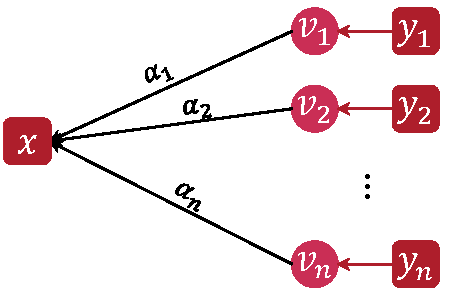
\includegraphics[width=0.45\linewidth]{figs/sensory_retrieval.pdf}
  \hfill
  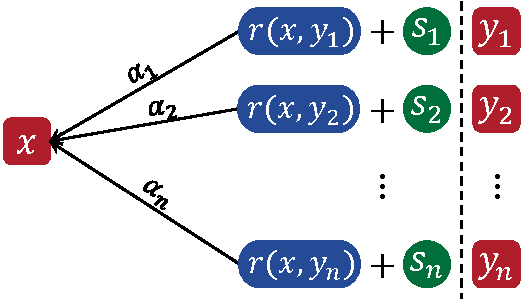
\includegraphics[width=0.45\linewidth]{figs/relational_retrieval.pdf}
  \caption*{Left: \senscolor{Sensory attention} retrieves object features. Right: \relcolor{Relational attention} retrieves relation vectors tagged with \symbcolor{symbols}}
\end{figure}



\relcolor{\textbf{\textit{\underline{Relational Attention}}}}: An attention mechanism for explicitly routing \emph{relational} information:
  \[\relcolor{\bm{a}_i} \gets \sum_{j} \attncolor{\alpha_{ij}} \cdot \paren{W_r \, \relcolor{\bm{r}_{ij}} + W_s \, \symbcolor{s_{j}}}\]

\begin{enumerate}
  \item \emph{Attend:} Compute \attncolor{\emph{attention scores}} to select object(s) to attend to
  \[\attncolor{\alpha_{ij}} = \mathrm{Softmax}([\iprod{\phiqattn(\senscolor{x_i})}{\phikattn(\senscolor{x_j})}]_{j=1}^{n})_j\]


  \item \emph{Relate:} Compute \relcolor{\emph{relation vectors}} representing relationship with attended object(s)
  \[\relcolor{\bm{r}_{ij}} = \paren{\iprod{\phiqrell{\ell}(\senscolor{x_i})}{\phikrell{\ell}(\senscolor{x_j})}}_{\ell \in [d_r]} \in \reals^{d_r}\]

  \item Tag with \emph{\symbcolor{symbols}}: Abstract \symbcolor{identifiers}
  \[(\symbcolor{s_1}, \ldots, \symbcolor{s_n}) = \SymbolRetriever(\senscolor{x_1}, \ldots, \senscolor{x_n})\]
\end{enumerate}

\begin{center}\rule{0.9\linewidth}{0.5pt}\end{center} % divider

\mixedcolor{\textbf{\textit{\underline{Dual Attention:}}}} A \emph{multi-head} attention mechanism consisting of a \emph{combination} of \emph{\textbf{standard attention}} heads---for attending to \emph{\senscolor{sensory}} information---and \textbf{\emph{relational attention}} heads---for attending to \emph{\relcolor{relational}} information.

% \begin{center}\rule{0.9\linewidth}{0.5pt}\end{center} % divider

\mixedcolor{\textbf{\textit{\underline{Dual Attention Transformer (DAT):}}}} A Transformer architecture where each \emph{multi-head attention} module is replaced with \emph{\mixedcolor{dual attention}}, enabling explicit joint routing of both sensory and relational information.

\end{block}

\end{column}

\separatorcolumn

\begin{column}{\colwidth}

\begin{block}{Highlights of Experimental Results}

    \textbf{Mathematical Problem Solving (Seq2Seq)}
    \begin{figure}
        \centering
        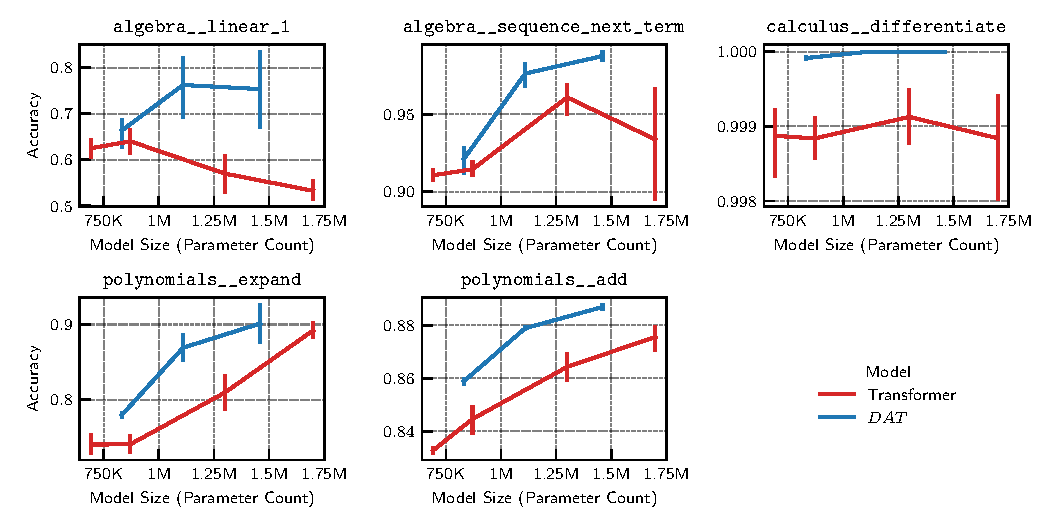
\includegraphics[width=\linewidth]{figs/experiments/math/math_accuracy_scaling.pdf}
        \caption*{\mixedcolor{\emph{DAT}} shows superior scaling on mathematical reasoning tasks}
    \end{figure}

    \textbf{Language Modeling Scaling Laws}
    \begin{figure}
        \centering
        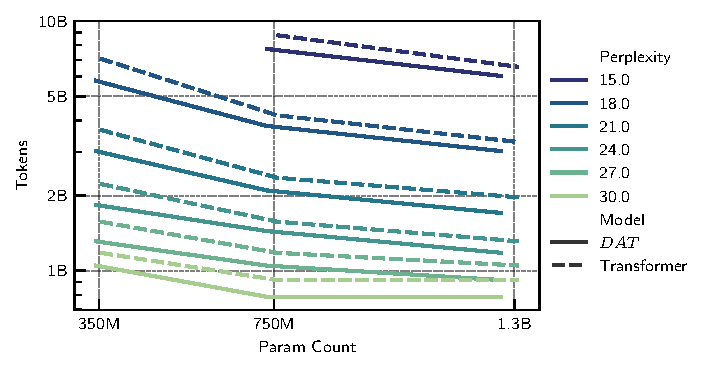
\includegraphics[width=0.85\linewidth]{figs/experiments/fineweb/tokens_vs_param_count.pdf}
        \caption*{\mixedcolor{\emph{DAT}} is more data-efficient and parameter-efficient than standard Transformers}
    \end{figure}

  \textbf{Visualization of Learned Latent Relational Representations}
  \begin{figure}[t]
    \centering
    \begin{subfigure}[t]{\textwidth}
        \centering
        \scalebox{-1}[-1]{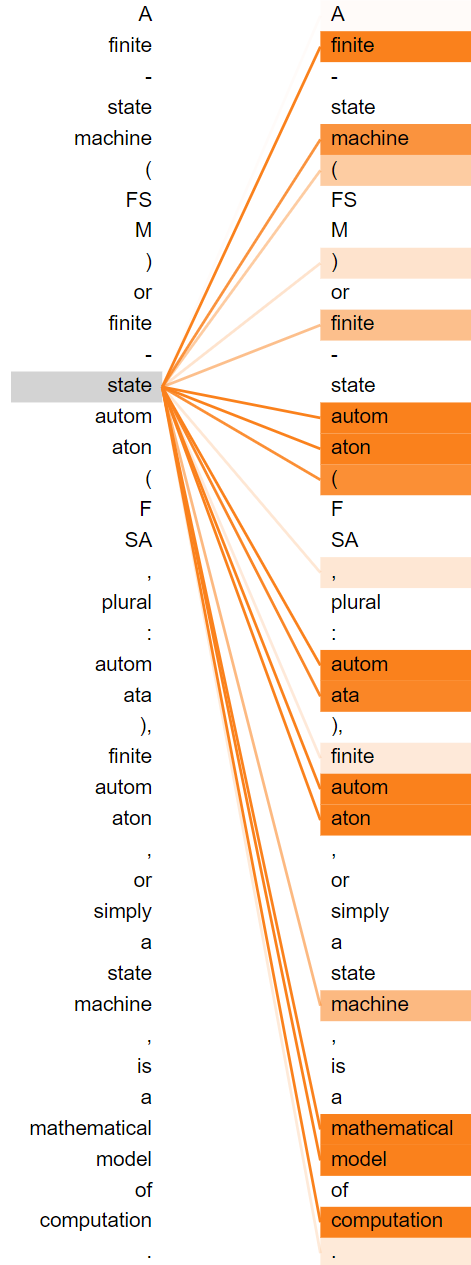
\includegraphics[height=0.8\textwidth, angle=-90]{figs/experiments/fineweb/viz/DAT-343M-viz-L12-rel2-state.png}}
        % \caption{}\label{fig:}
    \end{subfigure}
    \caption*{A visualization of the learned relation activations in a \emph{DAT} language model. This depicts one dimension of the relation vector $\relcolor{\bm{r}_{ij}}$ in the twelfth layer, focusing on the token \texttt{`state'} as the source $i$, which has high activation with the tokens \texttt{`mathematical'}, \texttt{`model'}, and \texttt{`computation'}.}
    % \vskip-8pt
\end{figure}
\end{block}

\end{column}

\separatorcolumn
\end{columns}
\end{frame}

\end{document}